\documentclass[a4paper,11pt]{article}
\pdfoutput=1 % if your are submitting a pdflatex (i.e. if you have
             % images in pdf, png or jpg format)

\usepackage{jcappub} % for details on the use of the package, please
                     % see the JCAP-author-manual

\usepackage[T1]{fontenc} % if needed
% \usepackage{subfig}
\usepackage[utf8]{inputenc}

\usepackage{color}
\usepackage[toc,page]{appendix}

\newcommand{\ek}[1]{{{\bf \color{red} EK: #1}}}
\newcommand{\re}[1]{{{\bf \color{green} RE: #1}}}

\title{\boldmath The Core-Cusp Problem Revisited: ULDM vs. CDM}


%% %simple case: 2 authors, same institution
%% \author{A. Uthor}
%% \author{and A. Nother Author}
%% \affiliation{Institution,\\Address, Country}

% more complex case: 4 authors, 3 institutions, 2 footnotes

\author[1]{Emily Kendall,}
\author[1]{Richard Easther}


% The "\note" macro will give a warning: "Ignoring empty anchor..."
% you can safely ignore it.

\affiliation[1]{Department of Physics, University of Auckland, Private Bag 92019, Auckland, New Zealand}

% e-mail addresses: one for each author, in the same order as the authors
\emailAdd{eken000@aucklanduni.ac.nz}
\emailAdd{r.easther@auckland.ac.nz}




 
\abstract{The core-cusp problem is often cited as a motivation for the exploration of dark matter models beyond standard CDM [cold dark matter]. One such alternative is ULDM [ultra-light dark matter]; particles exhibiting wavelike properties on kiloparsec scales. ULDM dynamics are governed by the Schr\"{o}dinger-Poisson equations,  which have solitonic ground state solutions consisting of gravitationally-bound condensates with no internal kinetic energy. Astrophysically realistic ULDM halos would  consist of larger NFW-like configurations with a possible solitonic core. We describe a parameterisation for the radial density profiles of ULDM halos that  accounts for the environmental variability of the core-halo mass relation. We then compare the semi-analytic profiles of ULDM and CDM with astrophysical data, and find that a ULDM particle mass of $10^{-23}\operatorname{eV}$ can yield a reasonably good fit to observed rotation data, particularly at small radii. This ULDM mass is in tension with other constraints but we note that this analysis ignores any contribution from baryonic feedback.}
 


\begin{document}
\maketitle
\flushbottom


\section{Introduction}\label{sec:intro}

 
It is widely agreed that non-baryonic dark matter constitutes the majority of the mass of the observable universe, but its precise nature remains an open question. Many dark matter models have been proposed, with particle CDM [Cold Dark Matter]  being the most widely studied. This scenario successfully accounts for the large scale structure of the universe \cite{Springel:2005nw} and the spectrum of anisotropies in the microwave background \cite{deBernardis:2000sbo, Hanany:2000qf, Halverson:2001yy, Netterfield:2001yq, Lee:2001yp, Ade:2015xua,  Hu:2001bc}, but the so-called ``small-scale crisis''  remains a challenge \cite{Weinberg:2013aya}. A key issue is the tension between the  central density profiles of dark matter halos in simulations containing only gravitationally interacting CDM, and those inferred from observational data. Simulations tend to produce `cuspy' central density profiles \cite{Navarro:1995iw}, which grow as $1/r$ at small radii, but observational data appears to favour flattened central cores \cite{Moore:1994yx}. This so-called core-cusp problem has been the focus of much recent attention \cite{Dutton:2018nop, Read:2018pft, Genina:2018}. 
 
The seriousness of the core-cusp problem is the subject of ongoing debate, and may be ameliorated by adding baryonic matter to CDM simulations \cite{Benitez-Llambay:2018}. Nevertheless, the wider category of  ``small-scale'' problems in standard CDM along with tighter constraints from direct-detection experiments \cite{Schumann:2019eaa} motivates the study of alternative dark matter models. One scenario which has gained substantial traction is ultra-light dark matter [ULDM], also known as scalar-field dark matter, $\Psi$ dark matter, axion dark matter, BEC dark matter and fuzzy dark matter. As reviewed by Hui {\em et al.\/} \cite{Hui:2016ltb}, ULDM consists of an axion-like particle whose very small mass  ($\mathcal{O}(\sim 10^{-22}eV)$) corresponds to a kiloparsec-scale de Broglie wavelength. ULDM thus exhibits novel wave-like behaviour on astrophysically interesting scales and can form soliton-like gravitationally confined Bose-Einstein condensates. ULDM simulations suggest that realistic astrophysical halos have an inner core consisting of a kiloparsec scale Bose-Einstein condensate or soliton, while the outer halo is a virialised system of scalar particles matching expectations from standard CDM \cite{Schwabe:2016rze, Veltmaat:2018dfz}. 

As the  centres of ULDM solitons are relatively flat it seems that ULDM could  resolve the CDM core-cusp problem without the inclusion of baryonic astrophysics. However, it has  been suggested that in some mass regimes ULDM actually exacerbates the core-cusp problem relative to the NFW [Navarro-Frenk-White] profiles  \cite{Navarro:1995iw} characteristic of WIMP [Weakly Interacting Dark Matter] CDM \cite{Robles:2018fur}. This is because the inner regions of ULDM halos are described by solitonic density profiles which obey a scaling law in which the width of the soliton scales inversely with its mass. Consequently, for massive cores it is plausible that the density of the ULDM halo might exceed that of an analogous NFW halo at small radii. The authors of Ref~\cite{Robles:2018fur} concluded that NFW profiles can actually outperform ULDM profiles for large dwarf galaxies (halo masses $M_h$ in the range $M_h \gtrsim 10^{11} M_{\odot}$).  

In this work we examine the scatter in the core-halo mass scaling relation and its implications for discussions of the core-cusp discrepancy in ULDM. Starting from the semi-analytic density profile of Ref.~\cite{Robles:2018fur} we look at the scatter in the parameters implied by Ref.~\cite{Schive:2014hza}, showing that this can ease concerns that the core-cusp problem is  exacerbated for ULDM relative to CDM for large dwarf galaxies. Furthermore, by numerically building ``synthetic'' halos through soliton mergers (using the {\sc PyUltraLight} code \cite{Edwards:2018ccc}) we see that while the spherically-averaged density profiles of simulated ULDM halos follow a predictable format, the incoherent outer regions fluctuate strongly, providing further evidence for the presence of intrinsic scatter in halo parameters at fixed mass although we emphasise that these analyses ignore baryonic feedback, which is known to be significant for dwarf galaxies \cite{2018MNRAS.473.5698D, Benitez-Llambay:2018}. We find that for dark matter-only models, neither ULDM halos (for ULDM particle mass $0.8-2.5\times 10^{-22} \operatorname{eV}$)
nor NFW halos provide an overwhelmingly convincing fit to rotation curves of large dwarf galaxies, suggesting significant contributions from baryonic physics would be necessary for either model to yield a good fit to data. Here we use the SPARC database \cite{Lelli:2016zqa} to obtain galactic rotation curves. The details of this database will be discussed in following sections, but the curves for some dwarf galaxies are limited to a few data points, and many profiles have significant uncertainties, further complicating attempts to draw robust conclusions from this approach. 

These uncertainties notwithstanding, we look at the subset of SPARC galaxies which exhibit a steep decrease in rotation velocity at small radii, and find that a ULDM particle mass of $10^{-23}\operatorname{eV}$ can yield a reasonable fit to this data without the inclusion of baryonic physics, suggesting the core-cusp problem is naturally ameliorated in this case. This  small ULDM particle mass, however, is in tension with some recent ULDM constraints. Hence, further investigation is needed to determine whether ULDM provides a suitable framework to describe dwarf galaxies.  

The structure of the paper is as follows. In Section \ref{sec:models}, we review the construction of semi-analytic density profiles for both the ULDM and CDM models. In Section \ref{sec:sim_comparison} we briefly discuss aspects of realistic ULDM halos which are not captured by the semi-analytic model. In Section \ref{sec:velocity} we compare the semi-analytic density profiles for ULDM and CDM halos in the dwarf galaxy mass range $10^{11} - 10^{12}\operatorname{M}_{\odot}$, taking into account statistical variation in both the NFW concentration parameter and the ULDM core-halo mass relation. We then compare the radial velocity profiles inferred from these density profiles with astrophysical data from the SPARC database \cite{Lelli:2016zqa}. We conclude in Section \ref{sec:conclusion}.

\clearpage





\section{Semi-analytic models of dark matter halos}\label{sec:models}


\subsection{The NFW profile of CDM}\label{sec:NFW}

We begin by looking at the semi-analytic parametrisations of ULDM and CDM halo models. The  well known  NFW   profile of CDM \cite{Navarro:1995iw, Maccio:2008pcd}  is given by
%
\begin{equation}\label{eq:nfw}
    \rho_\mathrm{NFW}(r)=\frac{\rho_0}{\frac{r}{R_s}\left(1+\frac{r}{R_s}\right)^2} \, .
\end{equation}
%
The parameters $\rho_0$ and $R_s$ vary from halo to halo; $\rho_0$ can be interpreted as a characteristic density, while $R_s$ is the scale radius and determines the radius at which the transition between the `small $r$' and `large $r$' limits occurs. At small radii the profile is proportional to $1/r$, while at large radii it goes as $1/r^3$.

The NFW halo is assumed to be radially symmetric, and requires truncation at a finite radius in order to avoid the divergence in the mass integral as $r\rightarrow \infty$. This is typically set by the virial radius, which is approximately determined via the spherical top-hat collapse model \cite{White:2000jv, Suto:2015jdt, Herrera:2017epn} describing the evolution of a uniform spherical overdensity in a smooth expanding background. Gravitational collapse of the overdensity halts when virial equilibrium is reached. The corresponding virial radius is the radius at which the mean internal density is $\Delta_c \rho_\mathrm{crit}(t)$. Here $\rho_\mathrm{crit}(t)$ is the critical density of the universe at time $t$. The numerical factor $\Delta_c$ is of order $10^2$ and while different conventions exist, we will take the common value of $\Delta_c = 200$ \cite{Richings:2018} in what follows. 

Once the virial radius is specified as the outer limit of the halo, equation \ref{eq:nfw} completely specifies the density profile for given  $\rho_0$ and $R_s$. For any given virial mass, there is a range of corresponding NFW density profiles, with the distributions of $\rho_0$ and $R_s$ emerging from the mass-concentration-redshift relation seen in N-body simulations and observations \cite{Ludlow:2013vxa, Ragagnin:2018enf}. 

\subsection{The piecewise ULDM halo profile}

ULDM dynamics is governed by the Schr{\"o}dinger-Poisson system of coupled differential equations. In a static background, they take the dimensionless form  
%
\begin{align}
    i\dot{\psi} &= -\frac{1}{2}\nabla^2\psi+\Phi\psi \\
    \nabla^2\Phi &= 4\pi \vert \psi\vert^2
\end{align}
%
where $\psi$ is the ULDM wavefunction, $\Phi$ is the Newtonian potential, and the density $\rho \propto |\psi|^2$. The solitonic ground state profile cannot be written down analytically, but given a numerically computed spherically symmetric  profile $\psi$ with $\psi(0)=1$, the full family of solutions is
%
\begin{equation}
    \psi'(x) = \gamma\psi(\sqrt{\gamma}x),
\end{equation}
%
where $\gamma$ is a scaling parameter and the dimensionless mass of the soliton is proportional to $\sqrt{\gamma}$, while the dimensionless radius is proportional to $1/\sqrt{\gamma}$. The dimensionless density $\vert\psi\vert^2$ and dimensionless radius $x$ can be transformed into dimensionful quantities by
\begin{align}
    \rho &= \mathcal{M}\mathcal{L}^{-3}\vert\psi\vert^2, \label{eq:density_conv} \\
    r &= \mathcal{L}x, \label{eq:mass_conv}
\end{align}
where
\begin{equation}\label{eq:length}
    \mathcal{L}=\left(\frac{8\pi\hbar^2}{3 m^2H_0^2\Omega_{m_0}}\right)^{\frac{1}{4}}\approx121\left(\frac{10^{-23}\operatorname{eV}}{m}\right)^{\frac{1}{2}}\operatorname{kpc},
\end{equation}
%
and 
%
\begin{equation}\label{eq:mass}
    \mathcal{M}=\frac{1}{G}\left(\frac{8\pi}{3 H_0^2\Omega_{m_0}}\right)^{-\frac{1}{4}}\left(\frac{\hbar}{m}\right)^{\frac{3}{2}}\approx 7\times 10^7\left(\frac{10^{-23}\operatorname{eV}}{m}\right)^{\frac{3}{2}}\operatorname{M}_{\odot}.
\end{equation}

\

 
Ref.~\cite{Robles:2018fur} gives a piecewise parameterization of the generic ULDM profile 
%
\begin{equation}\label{eq:piecewise}
     \rho(r)=
    \begin{cases}
      \rho_{sol}(r), & 0\leq r \leq r_{\alpha} \\
      \rho_\mathrm{NFW}(r), & r_{\alpha}\leq r \leq r_{\mathrm{vir}},
    \end{cases}
\end{equation}
%
where $\rho_{sol}(r)$ is the appropriately scaled density profile of the ground state soliton solution. The contribution from the solitionic core and the overall virial mass  obeys a scaling relationship \cite{Schive:2014hza}, which sets the  central density, $\rho_c$, of a ULDM halo with virial mass, $M_{\mathrm{vir}}$.  This yields an expression relating the core size to the velocity dispersion, and finally to the halo virial mass.%
\footnote{The authors of \cite{Schive:2014hza} suggest the following general expression:
\begin{equation}
    M_c = \alpha \left(\vert E\vert/M\right)^{1/2},
\end{equation}
where the core mass $M_c$ is determined by the total energy, $E$, and the total mass of the halo, $M$ where $\alpha$ is a constant of order unity. They then explain that the right hand side of the equation represents the halo velocity dispersion, while the left hand side  represents the inverse core size due to soliton scaling laws. By invoking the virial condition of the spherical collapse model, the authors then  construct the redshift dependent relationship between the solitonic core mass and the halo virial mass for a ULDM halo.}
%
The core-halo mass relation can also be understood simply by matching the virial velocities of the core and the wider halo (see Appendix \ref{app:core-halo} for details). 
At $z=0$ the relationship is found to be \cite{Schive:2014hza} 
%
\begin{equation}\label{eq:central_dens}
    \rho_c = 2.94\times10^6 \operatorname{M}_{\odot}\operatorname{kpc}^{-3}\left(\frac{M_{\mathrm{vir}}}{10^9 M_{\odot}}\right)^{4/3}m_{22}^{2}
\end{equation}
and 
\begin{equation}
    r_c = 1.6 \operatorname{kpc}\left(\frac{M_{\mathrm{vir}}}{10^9 M_{\odot}}\right)^{-1/3}\frac{1}{m_{22}},
\end{equation}
%
where $r_c$ is the radius at which the density is half of the central value, and $m_{22}$ is given by $m_{22} \equiv m / 10^{-22} \operatorname{eV}$ where $m$ is the ULDM particle mass. 

This approach gives a baseline profile for ULDM halos, but for a given virial mass we should in fact expect a range of possible central densities (one might consider this in some sense analogous to the scatter in NFW concentration parameters \cite{Maccio:2008pcd}). Indeed, numerical results \cite{Schive:2014hza} indicate a scatter of up to $\pm 50\%$ in the core mass $M_c$. Furthermore, the cores are not exact soliton solutions of the Schr\"{o}dinger-Poisson equation as they interact with the NFW-like outer halo, and as such their central densities can vary with time by as much as a factor of two \cite{Veltmaat:2018dfz}. Thus, the core-halo mass relation should not be interpreted as an inviolable rule, but rather a statement about the averaged characteristics of a statistical distribution. Moreover, theoretical expectations for this distribution are currently poorly characterised, as high-fidelity ULDM simulations are computationally challenging. The small sample size and limited halo mass range ($ M_{\mathrm{vir}} \approx 10^8-10^{11} \operatorname{M}_{\odot}$) of the data in Ref.~\cite{Schive:2014hza} means it is probably not meaningful to use it to deduce the detailed statistical distribution of astrophysical halos. Furthermore, one must be cautious when extrapolating the core-halo mass relation to realistic halos in regions of parameter space which have yet to be explored numerically. It is difficult to accurately predict, for example, the effect that star formation and feedback will have on the formation of solitonic cores in halos of different masses, though one expects this effect to be significant at small radii. With the limitations of DM-only models in mind, we will  assume a scatter of $\pm 50\%$, noting that future simulations which include baryonic feedback will hopefully lead to improved predictions for this distribution. 

In addition to the variation in peak core density, we expect to see variation in the radius at which the solitonic profile of the ULDM halo transitions into an NFW profile. This is acknowledged in \cite{Robles:2018fur}, and is captured by the parameter $\alpha$, such that the transition radius, $r_{\alpha}$, is given by $r_{\alpha} = \alpha r_c$, where $3 \leq \alpha \leq 4$. The chosen value of the radius of transition will of course affect the parameters of the theoretical outer NFW halo, in particular the scale radius, as the core-halo mass relation should be maintained as the transition radius is varied.

With the allowances for statistical variation in both the central soliton density and the transition radius taken into account, we can create a range of plausible ULDM halo profiles for a given halo virial mass. To do this, we use the virial mass to predict $\rho_c$, and then allow the range of densities within $\pm 50\% $ of this central value. Combining the central density with an assumption for $\alpha$, the solitonic piece of the ULDM profile is then completely specified, and its mass can be calculated. From here, we can calculate the remainder of the virial mass which must be accounted for by the NFW tail of the profile, and by matching the densities of the NFW tail and the inner soliton at the transition radius, the values of the $R_s$ and $\rho_0$ parameters of the ULDM profile NFW tail are fully constrained.  



\section{Substructure in simulated ULDM halos}\label{sec:sim_comparison}

Halo formation in the ULDM model has been investigated in a number of studies \cite{Schwabe:2016rze, Mocz:2017wlg, Lin:2018whl}. These suggest that a `generic' ULDM halo consists of a solitonic core surrounded by an incoherent outer region whose density profile resembles that of an NFW halo, as described in the previous Section. Full astrophysical structure formation simulations in ULDM are particularly challenging, given the need to effectively resolve a wide range of scales in an expanding background. However, we can produce ``synthetic'' halos by initialising a Schr{\"o}dinger-Poisson solver so that it contains ${\cal{O}}(10)$ randomly located solitons, allowing them to merge and running the simulation long enough to arrive at a stable ``final'' state \footnote{We note that halo formation from solitonic mergers differs significantly from halo formation through direct gravitational collapse, and we must therefore be cautious when extrapolating results from one regime to the other}. 

We implemented this approach in {\sc PyUltraLight} \cite{Edwards:2018ccc}, and the results of one such simulation are shown in Figure \ref{fig:pul}. This profile is the result of the merger of eight randomly positioned solitons, yielding in a final profile with central density $\sim 10^{11}$ code units. The simulation was run at $512^3$ for a duration of 0.05 code units, while the volume of the simulation region, also in code units, was $0.2^3$.  The solitons were initially within the innermost eighth of the total simulation region, ensuring the periodic boundary conditions do not  prevent inward gravitational collapse. Halos produced this way cannot be expected to accurately reproduce astrophysical configurations, as their formation history differs greatly from the collapse of initially small overdensities that characterises cosmological structure formation. Moreover, this simulation has no expansion, so the critical density is ill-defined and  cannot be correlated with a virial overdensity, as outlined in Section \ref{sec:NFW}. Finally, resolving the central soliton restricts us to a simulation volume which cannot encompass the full virial radius of a given halo. Consequently, this is qualitative illustration of a ULDM halo, rather than a quantitative analysis. The conversion of dimensionless code units to physical units is a function of the ULDM particle mass and thus a particular set of simulation parameters could correspond to a range of physical parameters. However, for a general indication of scale, note that when a ULDM particle mass of $10^{-22}\operatorname{eV}$ is assumed, the above code parameters would correspond to a final halo mass of $\sim 10^{13}\operatorname{M}_{\odot}$ (though most of this mass would not be expected to be retained within the simulation volume), central density of $\sim 4\times 10^{12} \mathrm{M}_{\odot}\mathrm{kpc}^{-3}$, simulation duration $\sim 3.8 \operatorname{Gyr}$, and side length $\sim 7.7 \operatorname{kpc}$.

\begin{figure}
\begin{tabular}{cc}
{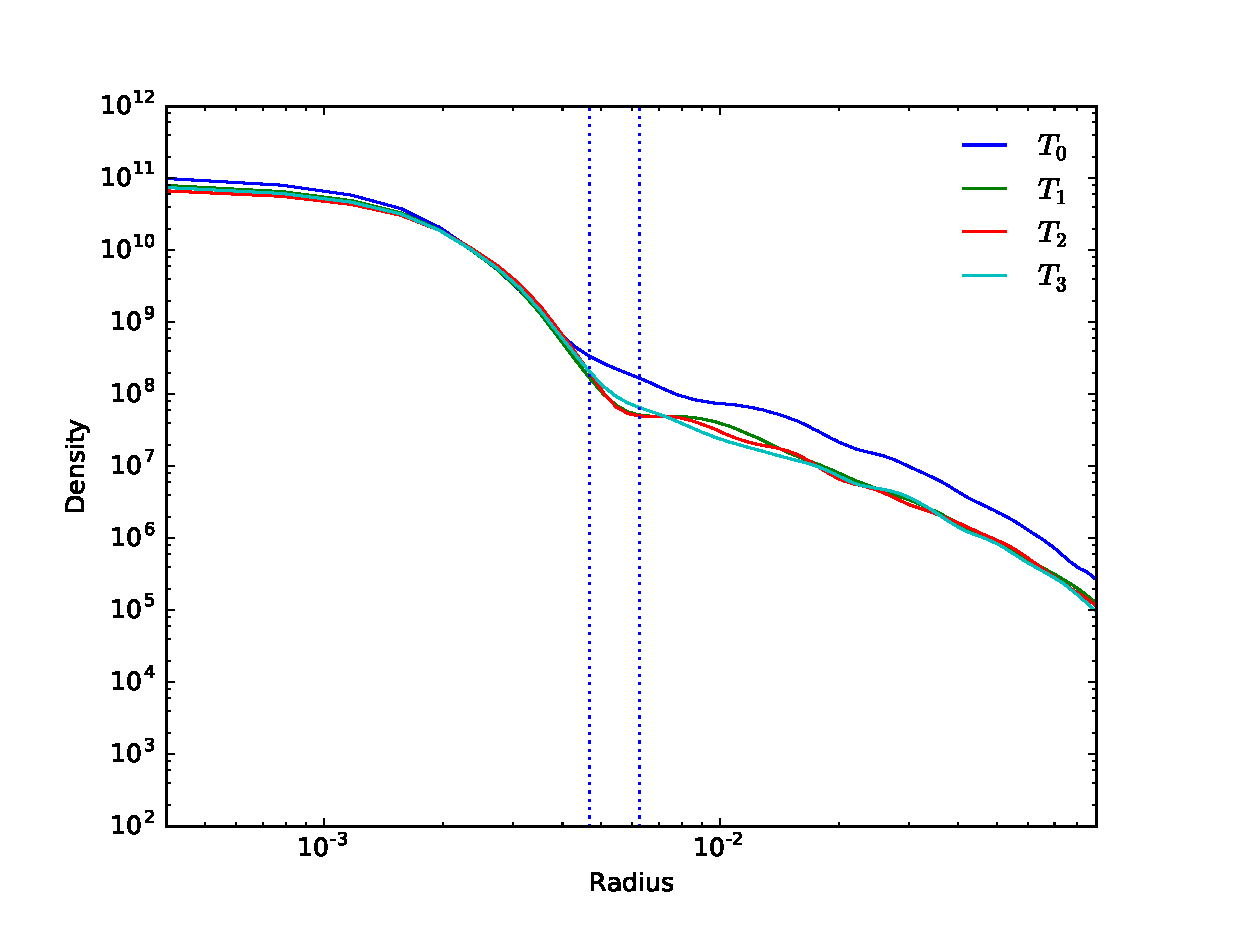
\includegraphics[scale = 0.42, trim={1.5cm 0 0 1cm}]{pics/M_comb.eps}} &
{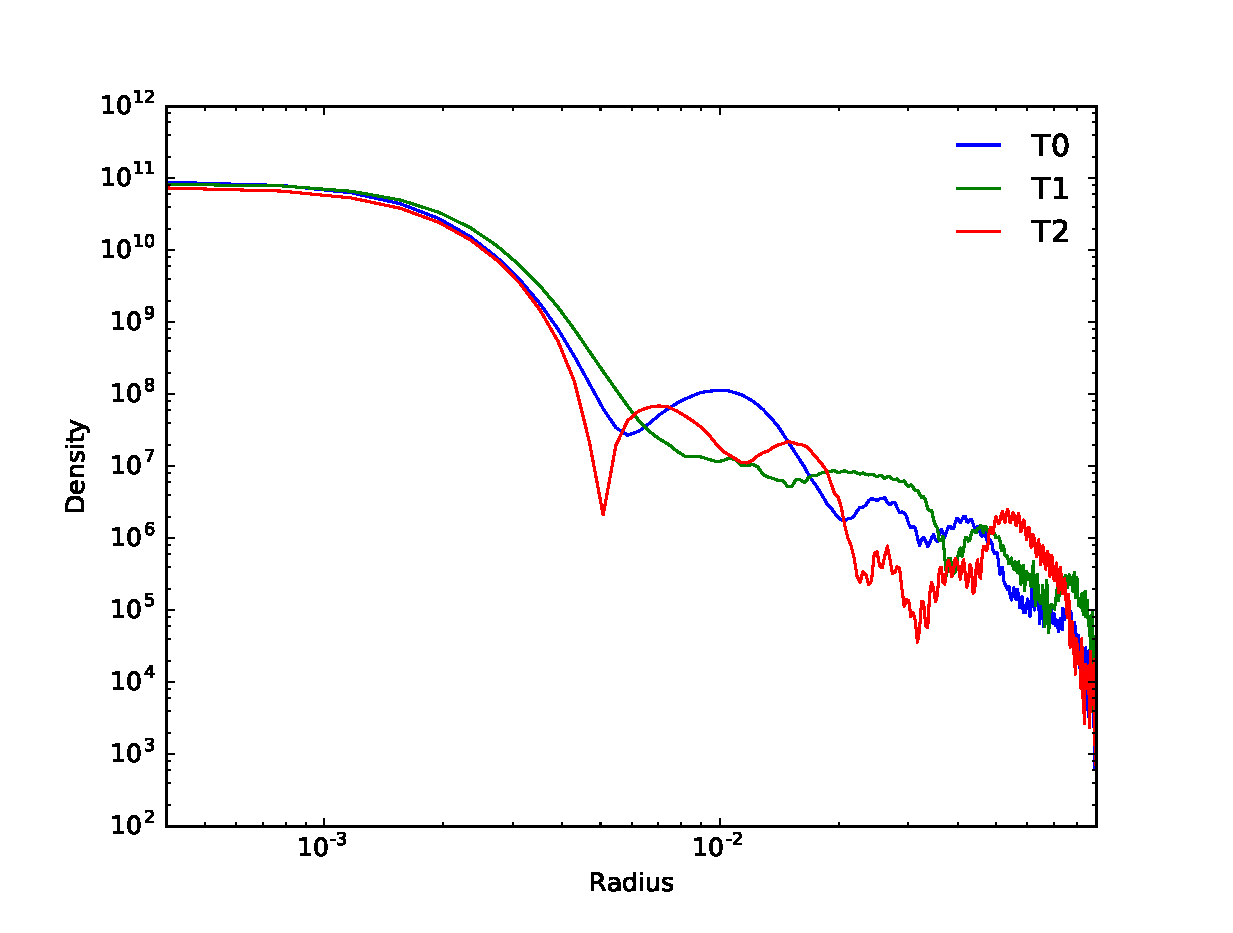
\includegraphics[scale = 0.42, trim={2.5cm 0 0 1cm}]{pics/M_singles.eps}}
\end{tabular}
\caption{Left: Spherically averaged density profile of late-time relaxed merger product of 8 solitons ($T_1$ - $T_3$). Also included is a profile before relaxation is complete, demonstrating an excess of mass in the inner halo ($T_0$). Vertical dotted lines represent 3 and 4 times the core radius. 
Right: Density profile along a single arbitrary direction for the relaxed halo at late times. All quantities are represented in dimensionless code units}\label{fig:pul}
\end{figure}

The left panel of Figure \ref{fig:pul} demonstrates the typical spherically-averaged relaxed halo profile obtained through solitonic mergers ($T_1$ - $T_3$). To obtain relaxed profiles,
{\sc PyUltraLight} was modified to include a sponge at the simulation boundary so that material ejected with large kinetic energy does not re-enter the box from the other side due to the periodic boundary conditions. Once the mass loss from the simulation region has asymptotically approached zero, a stable relaxed profile is obtained\footnote{Note that on the timescales considered here, it is difficult to see the fluctuations of the central density mentioned previously, which occur on much shorter timescales. For quantification of this effect, see \cite{Veltmaat:2018dfz}}. The shape of this overall profile remains similar as progenitor masses are increased/decreased, with a solitonic core (consistent with the inverse mass-radius scaling relation of the ground-state solution to the Schr{\"o}dinger-Poisson equations) transitioning to a $1/r^3$ type profile at a distance of between 3 and 4 times the core radius\footnote{Since mass is not globally conserved in these simulations and interactions between the outer halo and the inner region are not accounted for, we do not expect the profile to match the theoretical predictions for a cosmologically realistic virialised halo.}. Times $T_1$, $T_2$, and $T_3$ represent 90, 95, and 100$\%$ of the simulation duration, respectively. We also include one profile of the halo prior to relaxation for comparison ($T_0$ - 25\% of simulation duration), where we see an excess of mass in the inner halo. 

While the left panel of Figure \ref{fig:pul} shows spherically-averaged profiles, the right panel demonstrates that there are significant local fluctuations, both temporally and spatially, in the outer halo along any specific direction. The scale of these fluctuations is similar to that of the core itself, as can be seen in Figure \ref{fig:contour}, consistent with the non-local uncertainty principle invoked in Ref.~\cite{Schive:2014hza}. The implications of these fluctuations for local tracer velocities have been studied elsewhere \cite{Marsh:2018zyw} and they can provide a benchmark for comparing ULDM halo fluctuations to CDM substructure, as well as adding scatter to the expected velocity dispersion. We remark that these fluctuations are not captured by the semi-analytic model of ULDM halos, and that the consequences of this should be kept in mind when trying to fit such a model to observational data. In particular, in cases where velocities of only a small number of tracers within an astrophysical halo are known, it would be difficult to get an accurate idea of the average profile as local fluctuations may significantly affect individual tracers. 

\begin{figure}
\centering
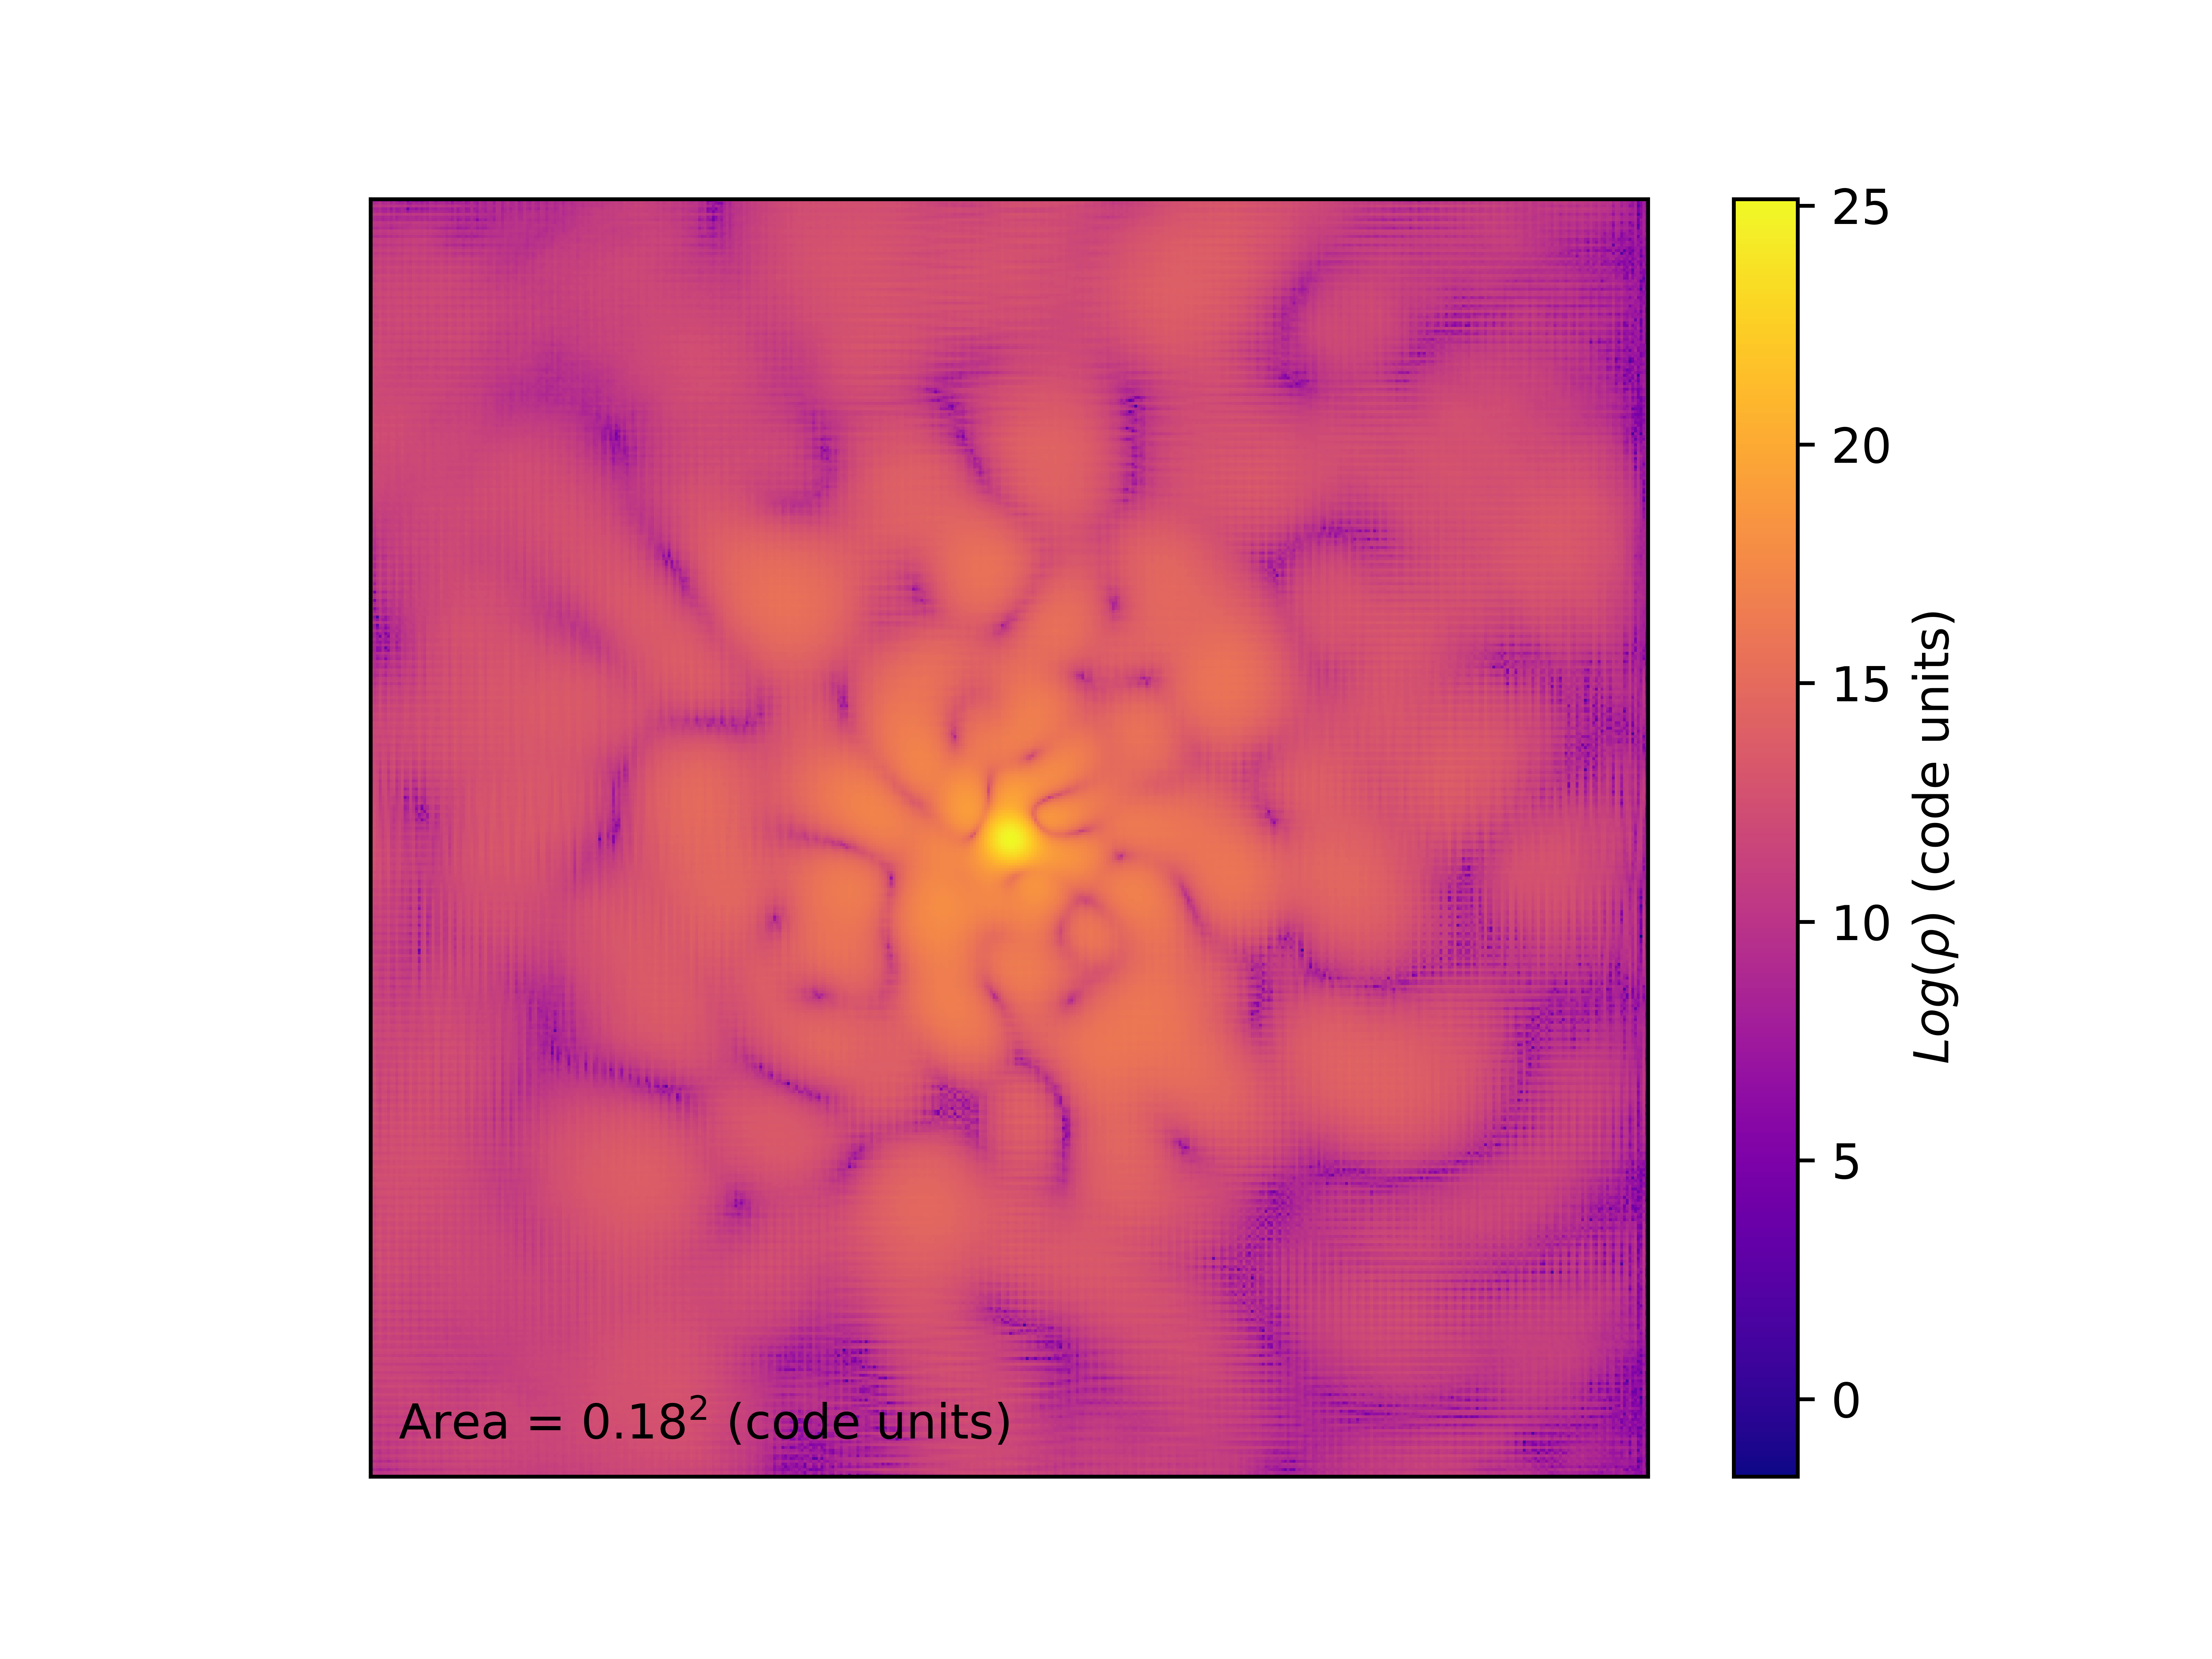
\includegraphics[scale = 0.7, trim={0cm 0cm 0cm 0cm}]{pics/slice.eps}
\caption{Illustration of the scale of the fluctuations present in the incoherent outer halo for the merger product of Figure \ref{fig:pul}. The contour plot represents the ($\mathrm{log}_{10}$ scaled) local density across a slice through the centre of the final halo. In this plot, distance is not log-scaled, and we see that the spatial size of the fluctuations is of the same order of magnitude as the solitonic core itself.}\label{fig:contour}
\end{figure}


\section{ULDM and CDM halos and astrophysical data}\label{sec:velocity}

 
Using the semi-analytic profiles described above, we now compare the radial profiles of ULDM halos to NFW halos. We focus on masses in the range $10^{11}$ and $10^{12} \operatorname{M}_{\odot}$ since these cases showed an apparent worsening of the core-cusp problem in Ref.~\cite{Robles:2018fur}. Figure \ref{fig:profiles} shows comparisons for representative masses; the green lines represent the ULDM density profiles at the extreme ends of the $\operatorname{M}_c = \operatorname{M}_{\mathrm{cp}} \pm 50 \% $ range, where $\operatorname{M}_{\mathrm{cp}}$ is the theoretical predicition for the core mass. Thanks to the  Schr{\"o}dinger-Poisson soliton scaling relations, this mass range corresponds to a range of $ \gamma_p /4 \leq \gamma \leq 9\gamma_p/4$, where $\gamma_p$ is the theoretical prediction of the square root of the dimensionless central density, implying a large variation in the central density and widely varying predictions for the overall ULDM profiles. Meanwhile $\pm$1$\sigma$ and $\pm$2$\sigma$ ranges for NFW profiles with different concentrations are shown as red and blue dots, respectively \cite{Maccio:2008pcd}. 

Following Ref~\cite{Robles:2018fur}, we plot to a minimum radius of $r/r_{\mathrm{vir}} = 10^{-4}$ and for the same choices of $m_{22}$. We note in passing that for any $\operatorname{M}_{\mathrm{vir}}$, the NFW halo density at very small radii will inevitably exceed that of the ULDM halo, though the threshold for this transition may be arbitrarily small, and not observationally relevant. From Figure \ref{fig:profiles} we see that for halo masses of $10^{11}\operatorname{M}_{\odot}$ there is a wide range of $M_c$ for which the ULDM profile is less cuspy than its NFW counterpart. For a halo mass of $10^{12}\operatorname{M}_{\odot}$ and a ULDM particle mass $m_{22}=0.8$ the ULDM profiles are likewise less peaked than the corresponding NFW profile, but at higher particle mass ($m_{22}=2.5$) the  NFW profiles tend to be less peaked than corresponding ULDM profiles at radial distances in  the range $10^{-4}\leq r/r_{\mathrm{vir}} \leq 1$.

\begin{figure}
\begin{tabular}{cc}
{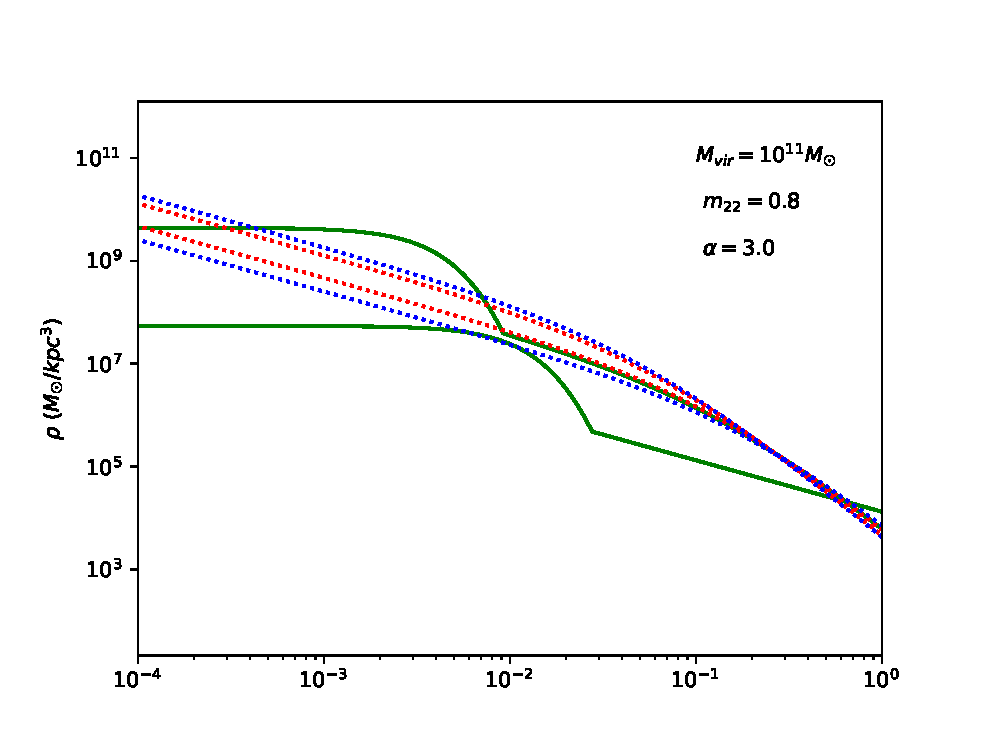
\includegraphics[width = 3.1in, trim={2.1cm 0.5cm 0cm 0.5cm}]{pics/11_8_3.eps}} &
{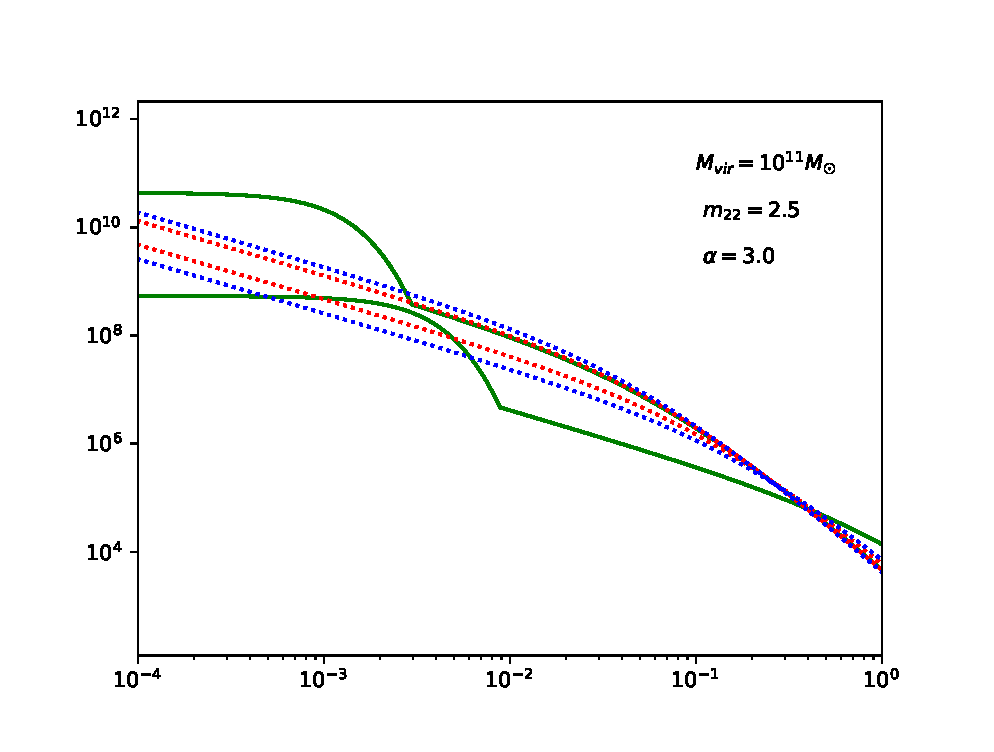
\includegraphics[width = 3.1in, trim={2.1cm 0.5cm 0cm 0.5cm}]{pics/11_25_3.eps}}\\
{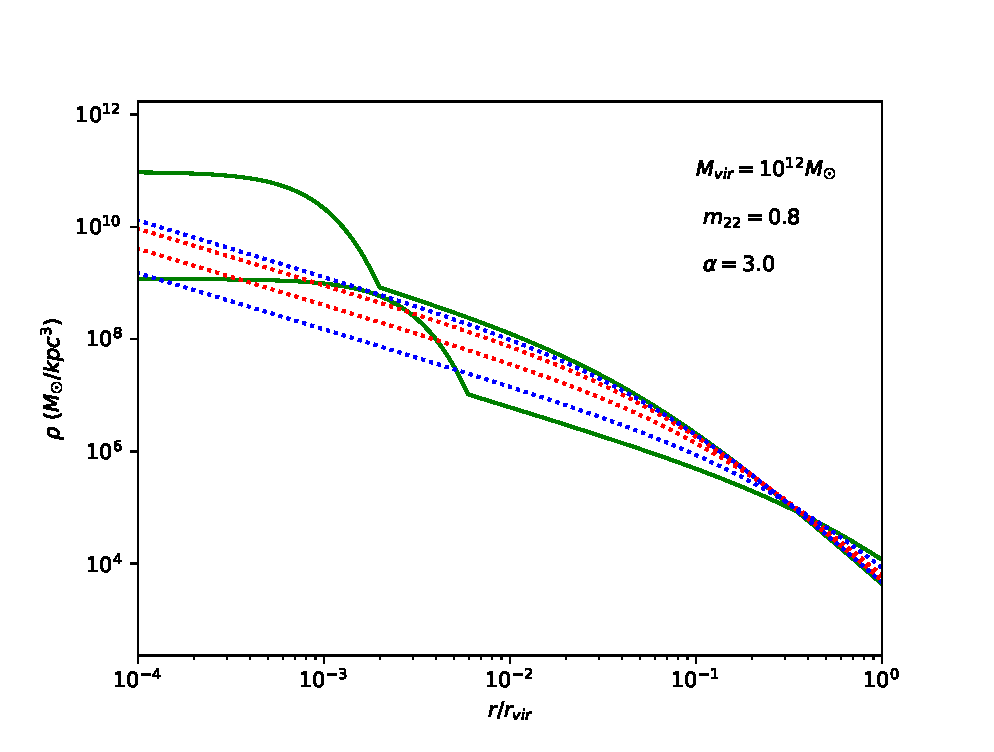
\includegraphics[width = 3.1in, trim={2.1cm 0.5cm 0cm 0.5cm}]{pics/12_8_3.eps}} &
{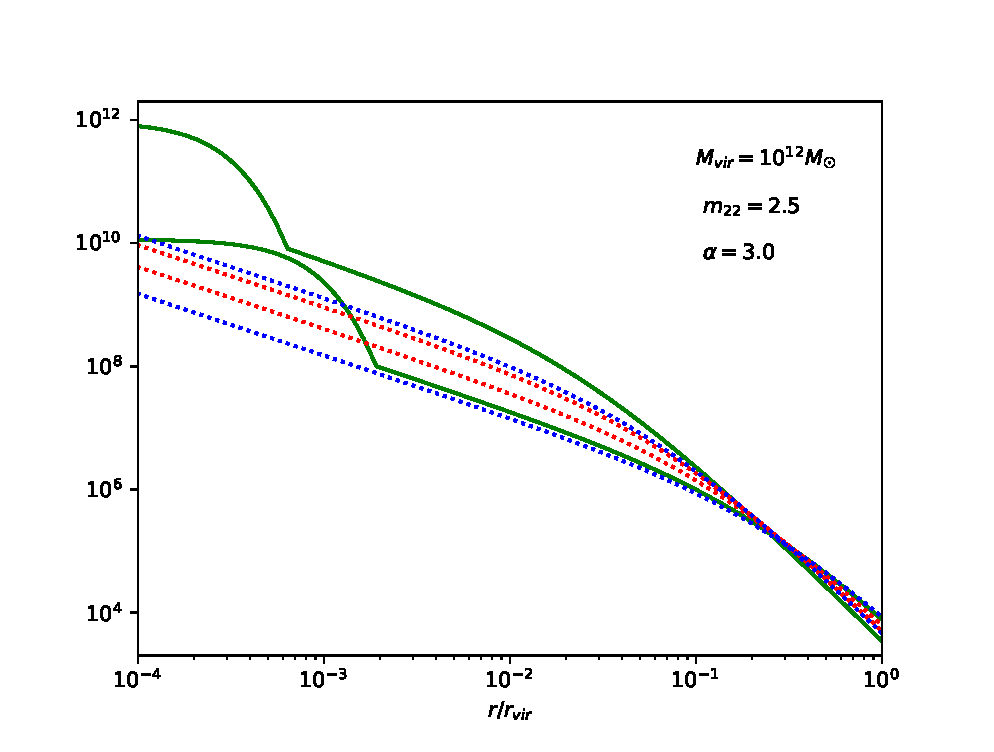
\includegraphics[width = 3.1in, trim={2.1cm 0.5cm 0cm 0.5cm}]{pics/12_25_3.eps}}
\end{tabular}
\caption{Density profiles as a function of radius (normalised to the virial radius) for ULDM and NFW halos of masses $10^{11}\operatorname{M}_{\odot}$ (top) and $10^{12}\operatorname{M}_{\odot}$ (bottom). The left panel represents the results for $m_{22} = 0.8$, while the right panel corresponds to $m_{22}=2.5$. The transition radius is fixed at $r_{\alpha} = 3*r_c$ as its value does not affect the value of the ULDM central density. Green lines represent  ULDM profiles with $\operatorname{M}_c = \operatorname{M}_{\mathrm{cp}} \pm 50 \% \operatorname{M}_{\mathrm{cp}}$.}\label{fig:profiles}
\end{figure}

It is not the dark matter halo density profiles themselves that are extracted from astrophysical observations, it is the radial velocity distributions of tracer stars. We convert our density profiles to radial velocity distributions \cite{Sofue:2008wt} via 
%
\begin{equation}
    V(r)^2 = \frac{4\pi G}{r}\int_0^r \rho(r')r'^2 dr',
\end{equation}
where 
\begin{equation}\label{eq:vel_decomp}
    V^2 = V_{\mathrm{disk}}^2 + V_{\mathrm{bulge}}^2 + V_{\mathrm{gas}}^2 + V_{\mathrm{halo}}^2.
\end{equation}
%


We now compare this distribution to profiles in the SPARC database, which contains photometric data for 175 galaxies and rotation curves from $\mathrm{H}_{\mathrm{I}}$/$\mathrm{H}_{\alpha}$ studies. The disk and bulge velocities in the SPARC database are given for $\Upsilon = 1 \operatorname{M}_{\odot}/\operatorname{L}_{\odot}$ at $3.6\operatorname{\mu m}$. However, the greatest source of uncertainty in mass modelling is the assumption for the stellar mass-to-light ratio, $\Upsilon_\star$ \cite{Lelli:2016zqa}. As in \cite{Robles:2018fur}, we  assume a constant value of $\Upsilon_\star = 0.2 \operatorname{M}_{\odot}/\operatorname{L}_{\odot}$ at $3.6\operatorname{\mu m}$, likewise noting that  this constitutes a non-trivial source of uncertainty. Moreover, there is significant uncertainty in the SPARC data itself, though the error bars are not plotted in the following graphs for ease of viewing. 

\begin{figure}
\begin{tabular}{cc}
{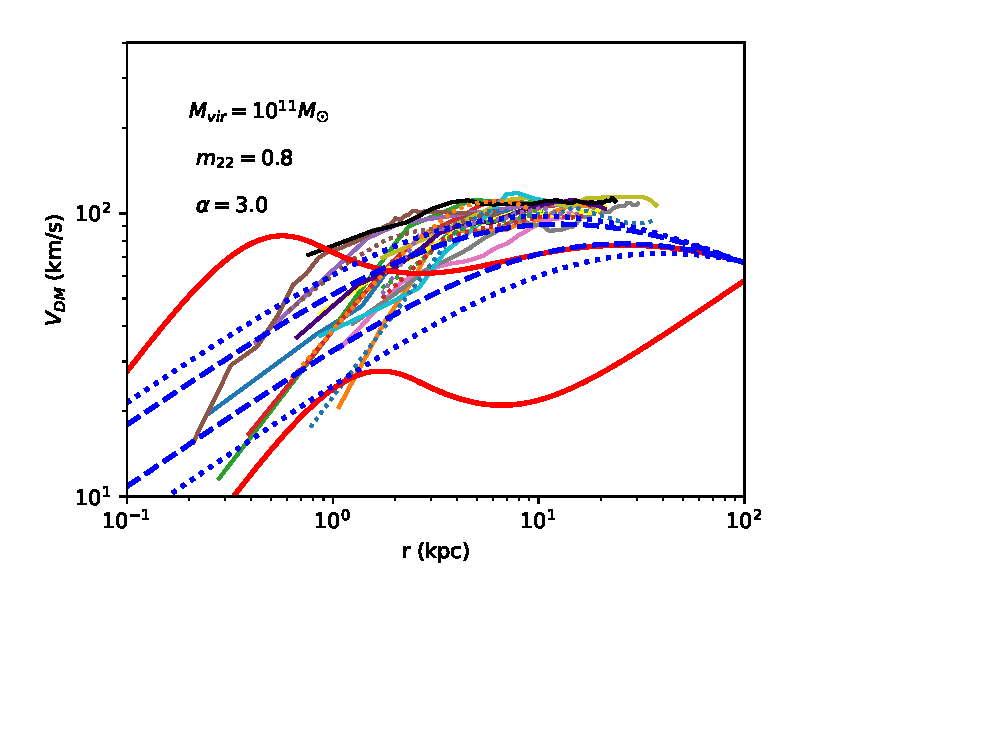
\includegraphics[scale = 0.65, trim={2.5cm 2.5cm 2.1cm 0.5cm}]{pics/v_11_8_3.eps}} &
{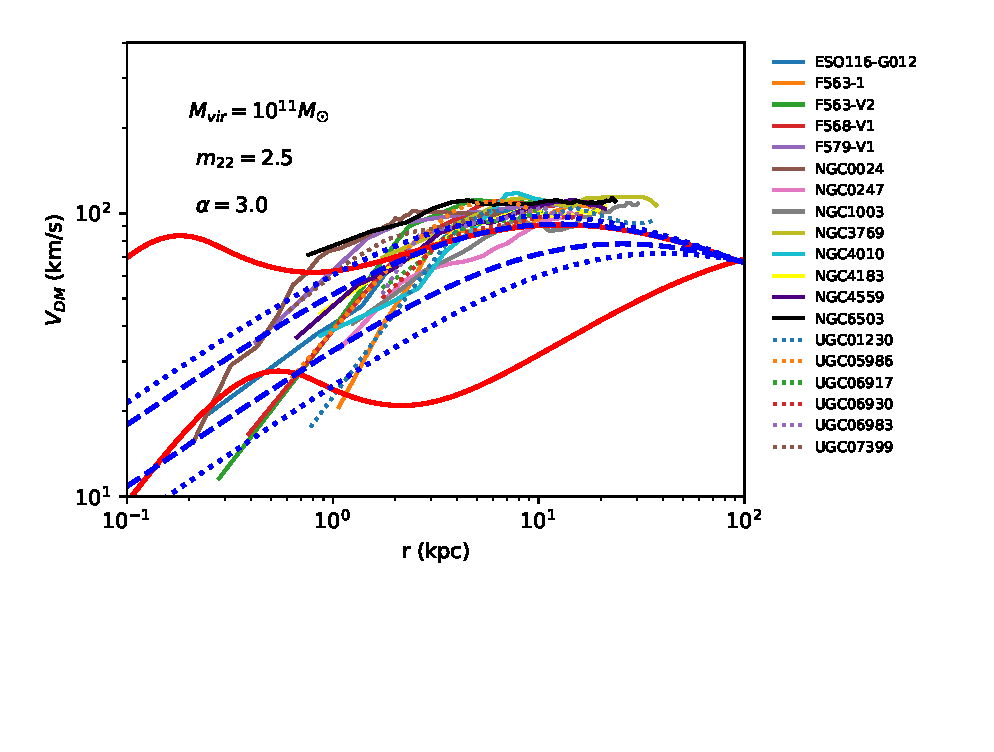
\includegraphics[scale = 0.65, trim={2.1cm 2.5cm 0cm 0.5cm}]{pics/v_11_25_3.eps}}
\end{tabular}
\caption{Theoretical NFW and ULDM velocity profiles for $10^{11}\operatorname{M}_{\odot}$ halos plotted against SPARC data filtered by $V_{\mathrm{max}} < 1.2 \operatorname{kms}^{-1}$. Red solid lines represent the extremal ULDM velocity profiles, while  blue dashed and dotted lines represent the 1-$\sigma$ and 2-$\sigma$ NFW bands, respectively. Results are shown for ULDM particle mass $m_{22} = 0.8$ (left) and $m_{22} = 2.5 $ (right). }\label{fig:velocity_11}
\end{figure}

\begin{figure}
\begin{tabular}{cc}
{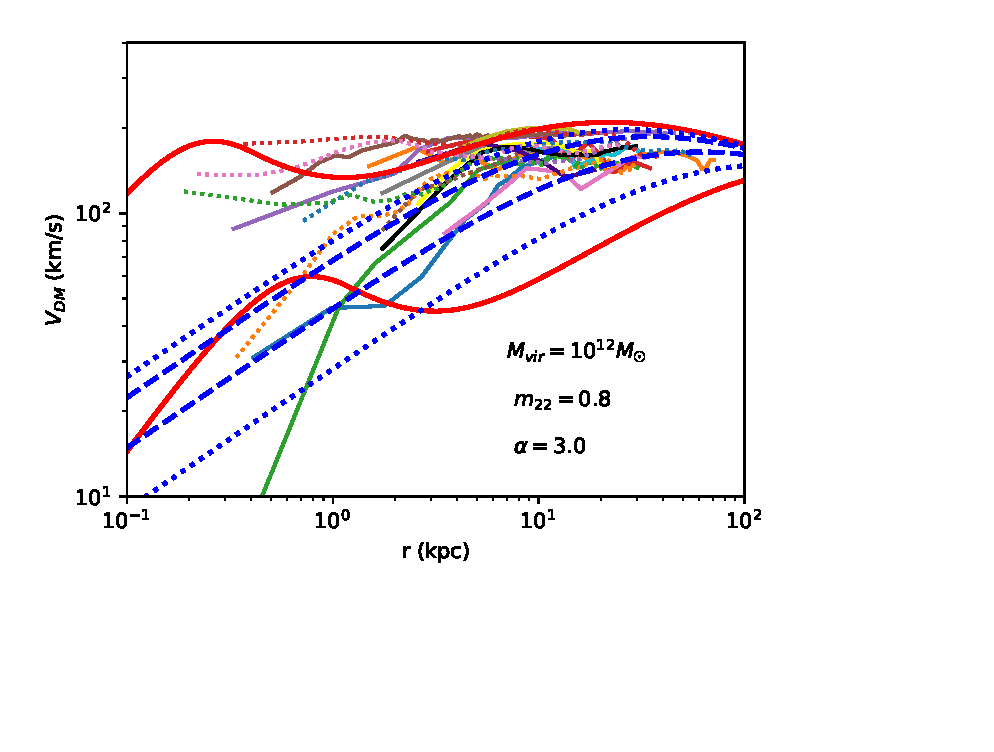
\includegraphics[scale = 0.65, trim={2.5cm 2.5cm 2.1cm 0.1cm}]{pics/v_12_8_3.eps}} &
{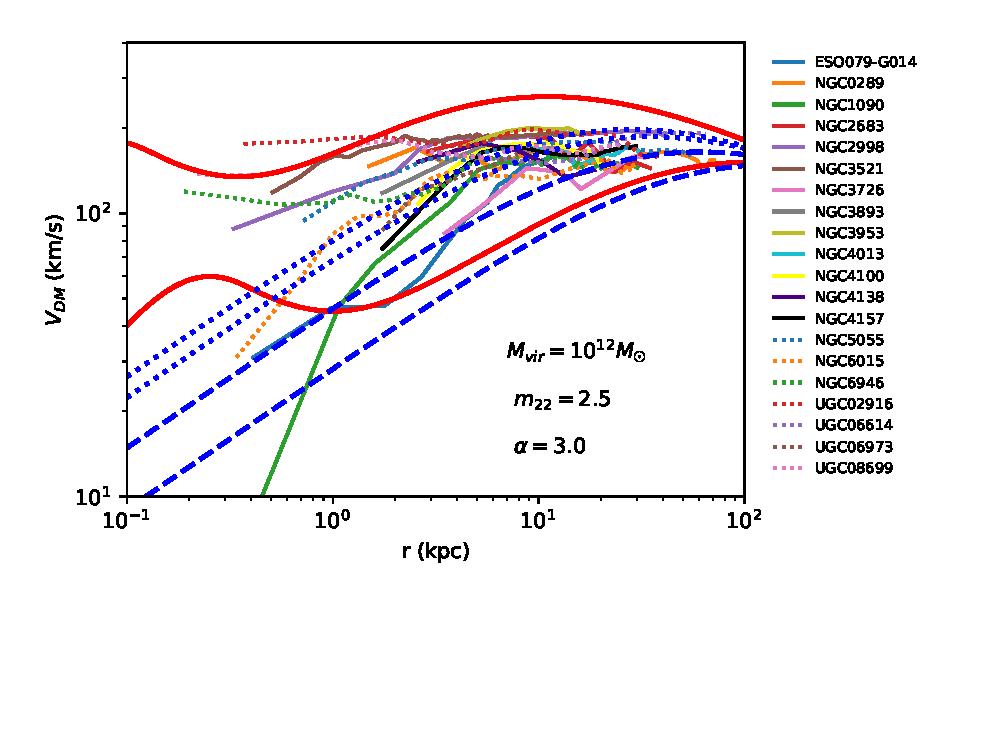
\includegraphics[scale = 0.65, trim={2.1cm 2.5cm 0cm 0.1cm}]{pics/v_12_25_3.eps}}
\end{tabular}
\caption{Theoretical NFW and ULDM velocity profiles for $10^{12}\operatorname{M}_{\odot}$ halos plotted against SPARC data filtered by $1.55\times 10^2 \operatorname{kms}^{-1}\leq V_{\mathrm{max}}\leq 2.0\times 10^2 \operatorname{kms}^{-1}$. Red solid lines represent the extremal ULDM velocity profiles, while  blue dashed and dotted lines represent the 1-$\sigma$ and 2-$\sigma$ NFW bands, respectively. Results are shown for ULDM particle mass $m_{22} = 0.8$ (left) and $m_{22} = 2.5 $ (right). }\label{fig:velocity_12}
\end{figure}


We consider the SPARC galaxies for which the outermost tracers have velocities $>100\operatorname{kms}^{-1}$. We can split this data into two rough categories; those which exhibit a strong steepening in the radial velocity profile toward the inner halo, and those which are comparatively flat. The former category corresponds to candidates for which the maximum velocity is roughly $< 1.2\times 10^2 \operatorname{kms}^{-1}$. The latter category corresponds to candidates for which the maximum velocity is roughly $1.55\times 10^2 \operatorname{kms}^{-1}\leq V_{\mathrm{max}}\leq 2.0\times 10^2 \operatorname{kms}^{-1}$ \footnote{We exclude data for which the velocities calculated according to Equation \ref{eq:vel_decomp} are inconsistent - this can occur due to the uncertainty in the assumption for $\Upsilon_\star$}. We will assume that higher asymptotic velocities correspond to a larger halo mass, and therefore expect a range of halo masses to be required to fit the data. We will consider halo masses in the range $10^{11} - 10^{12} \operatorname{M}_{\odot}$, expecting that masses at the top end of the range will be more suitable for modelling galaxies with higher asymptotic velocities. 

Our results are shown in Figures \ref{fig:velocity_11} and \ref{fig:velocity_12}. In Figure \ref{fig:velocity_11}, we see that assuming a halo mass at the lower end of the range ($10^{11}\operatorname{M}_{\odot}$) does not yield a good fit for the galaxies exhibiting a strong steepening of the inner velocity profiles. This is true for both NFW and ULDM profiles. While the core-cusp problem is not necessarily exacerbated in the ULDM case, ULDM profiles which roughly fit the data at low radii fall short at larger radii. This problem is worse at larger values of $\alpha$. That said, the proportion of baryonic matter is largest at the centre, so it is in this region that inaccuracies in the assumptions of the stellar mass to light ratio will be most critical. For this reason it is difficult to determine if either model is a good fit to the data. While the SPARC database does not contain any cases for which the velocity is significantly below $10^2\operatorname{kms}^{-1}$ at $10 \operatorname{kpc}$, it would appear that the ULDM profiles for the $10^{11}\operatorname{M}_{\odot}$ halos may provide a better fit to data in a lower velocity regime at this radius.



In Figure \ref{fig:velocity_12}, we show the comparison of the theoretical profiles for the $10^{12}\operatorname{M}_{\odot}$ halos with SPARC data satisfying $1.55 \times 10^2 \operatorname{kms}^{-1}\leq V_{\mathrm{max}}\leq 2.0 \times 10^2 \operatorname{kms}^{-1}$. While it would be difficult to find a universally applicable profile givien the variability in the trends shown by the data, there are a number of galaxies in this sample set which have flatter velocity profiles within the plotted range, such as NGC6946, UGC02916, and UGC08699. For these cases, the ULDM profile appears to provide a better fit, however more  data would be required to confirm this, particularly at small radii, where the ULDM and NFW profiles are expected to differ most. 


While the ULDM profiles predicted for $10^{11}\operatorname{M}_{\odot}$ halos at $m_{22} = 0.8 - 2.5$ do not provide convincing fits to this subset of SPARC data, the relatively high velocities at the outer radii suggest a slightly larger halo may provide a better fit. We test this possibility in Figure \ref{fig:velocity_23}. Here, we assume a ULDM halo mass of $5*10^{11}\operatorname{M}_{\odot}$, but do not obtain particularly good fits of the data for the ULDM particle mass range $m_{22} = 0.8 - 2.5$. Interestingly, however, if we assume a lower ULDM mass of $m_{22} = 0.1$ we find a much improved fit (the range of plausible halo velocity profiles for this choice of particle mass are shown by the solid black lines in Figure \ref{fig:velocity_23}). Figure \ref{fig:velocity_23} focuses on the smaller radii where the core-cusp discrepancy would be manifest and we see reasonable agreement with the velocities in these innermost regions under the assumption $m_{22} = 0.1$. It should be noted, however, that a ULDM particle mass of this magnitude is in tension with constraints from the Lyman-$\alpha$ forest \cite{Amendola:2005ad}, as well as high-redshift UV luminosity function comparisons \cite{Bozek:2014uqa}. Furthermore, we again emphasise that baryonic feedback would be of greatest significance in the innermost regions of realistic halos, and therefore such agreement between the semi-analytic model and the observational data should be interpreted cautiously. 



\begin{figure}
\centering
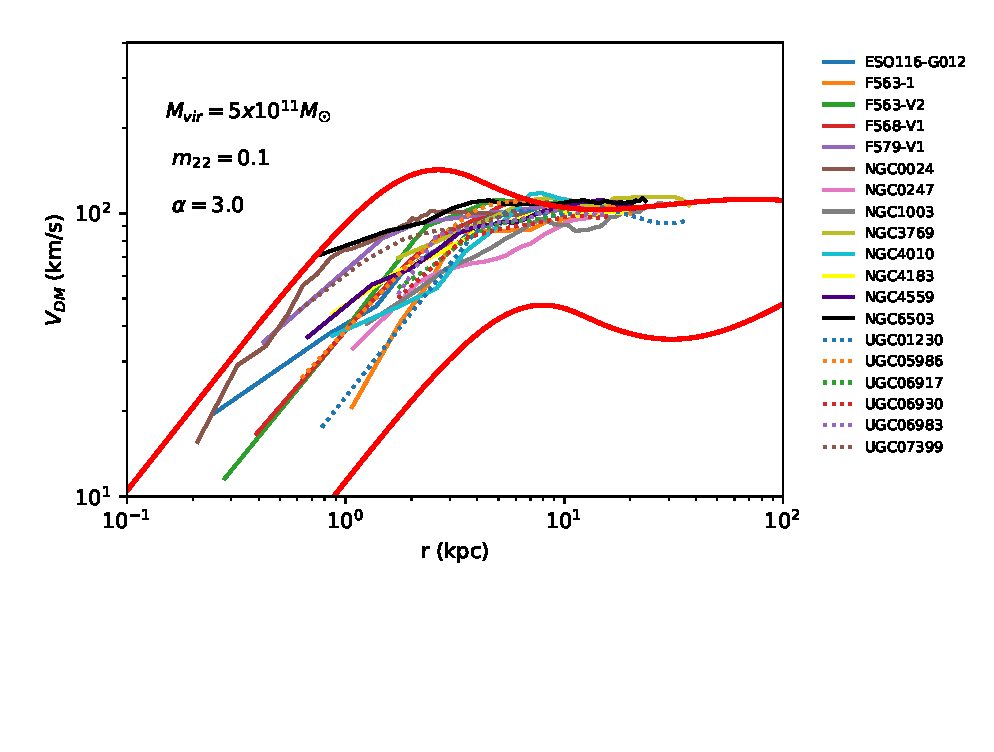
\includegraphics[scale = 0.8, trim={0cm 2.5cm 1cm 0.35cm}]{pics/best_match.eps} 
\caption{Range of theoretical ULDM profiles for a halo of mass $5\times 10^{11}\operatorname{M}_{\odot}$ with $m_{22} = 0.1$ (solid black lines), $m_{22} = 0.8$ (dotted black lines), and $m_{22} = 2.5$ (dashed black lines). Also plotted are the SPARC data satisfying $V_{\mathrm{max}}\leq 1.2\times 10^2 \operatorname{kms}^{-1}$. }\label{fig:velocity_23}
\end{figure}




\section{Conclusions}\label{sec:conclusion}

While the ULDM model has gained attention in part because it is a candidate solution to  the CDM core-cusp problem, in some cases ULDM profiles can have higher densities than their NFW counterparts at observationally relevant radii in the interior of massive dwarf galaxies. However, given the apparent spread in the predicted ULDM core-halo mass relation \cite{Schive:2014hza}, there is a sizeable range of plausible central densities for a halo of any given mass and analyses of oscillations of the cores of ULDM halos on timescales much smaller than the relaxation time have also demonstrated significant fluctuations in central density \cite{Veltmaat:2018dfz}. These observations suggest that the theoretical core-halo mass relation of ULDM should not be interpreted too literally for any individual halo, but is best viewed as a statistical feature of halo formation. In some circumstances, choosing a core mass at the lower end of the plausible range can mitigate the apparent core-cusp discrepancy.  

With the spread around the predicted core-halo relation in mind, comparison of theoretical ULDM and NFW profiles to photometric data from the SPARC database yields inconclusive results, as neither ULDM nor NFW profiles provide a particularly good fit to the data in the ranges $10^{11}\operatorname{M}_{\odot}\leq \operatorname{M}_{\mathrm{vir}} \leq 10^{12}\operatorname{M}_{\odot}$ and $0.8 \leq m_{22} \leq 2.5$. Interestingly, however, a better fit to the lower velocity SPARC data is obtained from a ULDM profile where $m_{22} = 0.1$ and $\operatorname{M}_{\mathrm{vir}} = 5\times 10^{11}\operatorname{M}_{\odot}$. It must be noted, however, that a ULDM  mass this small is in tension with other constraints \cite{Amendola:2005ad, Bozek:2014uqa, Armengaud:2017nkf, Ni:2019qfa, Nebrin:2018vqt}. Tightening these constraints on the plausible ULDM particle mass will inform future investigations of this type \cite{Castellano:2019hdd, Lidz:2018fqo, Davoudiasl:2019nlo}.


It is clear that more information, both from simulations and astrophysical observations, is required to fully explore the applicability of the ULDM model of dark matter. The parameter space used to describe ``typical'' ULDM halos appears to be larger than simple semi-analytical models would suggest, and must also ultimately include elements of baryonic feedback. Furthermore, a larger volume of photometric data with improved uncertainties  covering a greater halo mass range would be of tremendous benefit when testing dark matter scenarios, and can be expected from future surveys  \cite{Simon:2019kmm}. In addition, cosmological structure formation simulations for ULDM models continue to be an active area of research \cite{Lin:2018whl, Clough:2018exo, Mocz:2015sda}, which will improve the clarity of predictions for these scenarios.  This work thus emphasises the necessarily preliminary and tentative nature of all analyses of ULDM-derived rotation curves, and provides clear targets for future analyses. 


%check

\acknowledgments

We acknowledge invaluable discussions with Jens Niemeyer, Shaun Hotchkiss, and Mateja Gosenca in completing this work. We also acknowledge support from the Marsden Fund of the Royal Society of New Zealand. This research was supported by use of the Nectar Research Cloud, a collaborative Australian research platform supported by the National Collaborative Research Infrastructure Strategy (NCRIS).


\bibliographystyle{JHEP-mod}
\bibliography{refs} 


\begin{appendices}
\section{Core-halo mass relation}\label{app:core-halo}

The core-halo mass relation can be simply interpreted as the statement that the average internal velocity of a tracer mass in the core must be equal to the virial velocity of a tracer mass in the wider halo. If this were not the case, and instead the average velocity were higher within the core, these higher velocity particles would move outward, resulting in dynamical mass redistribution within the halo. During this process, the halo would not be in equilibrium and would thus not be virialised.

From the virial theorem we have that $E_K=-1/2 \ E_P$, where $E_K$ and $E_P$ represent kinetic and potential energies, respectively. Alternatively we can write:

\begin{equation}
    \frac{1}{2}M_{tot}v^2=\frac{1}{4}\frac{GM_{tot}^2}{R_{tot}},
\end{equation}
where $G$ is the gravitational constant, $M_{tot}$ and $R_{tot}$ are the total mass and radius, and $v^2$ is the mean of the squares of individual tracer velocities. Demanding that $v^2$ is the same for the core as for the total virialised halo allows us to then write
\begin{align}\label{eq:virial_cond}
    v^2&=\frac{GM_{\mathrm{vir}}}{2 R_{\mathrm{vir}}}=\frac{G M_{core}}{2 R_{core}}\nonumber\\
    &\rightarrow R_{core}=\frac{M_{core} R_{\mathrm{vir}}}{M_{\mathrm{vir}}}.
\end{align}
We know from the soliton scaling properties that $R_{core}\propto M_{core}^{-1}$, and since $M_{\mathrm{vir}}=4/3 \ \pi R_{\mathrm{vir}}^3 \Bar{\rho}$, we also have $R_{\mathrm{vir}} \propto M_{\mathrm{vir}}^{1/3}$. Hence, Equation \ref{eq:virial_cond} becomes
\begin{align}
    &R_{core}^2\propto \frac{R_{\mathrm{vir}}}{M_{\mathrm{vir}}}\nonumber\\
    &\rightarrow R_{core}^2\propto \frac{M_{\mathrm{vir}}^{1/3}}{M_{\mathrm{vir}}}\nonumber\\
    &\rightarrow R_{core}\propto\left(M_{\mathrm{vir}}^{-2/3}\right)^{1/2}\nonumber\\
    &\rightarrow R_{core}\propto M_{\mathrm{vir}}^{-1/3}.
\end{align}
With this scaling relation in mind, the constant of proportionality may be determined through analysis of simulated halos. 





\end{appendices}


\end{document}
